\documentclass{article}[12pt,letterpaper]
\usepackage{graphicx} % Required for inserting images
\usepackage{dirtytalk}
\usepackage{geometry}[margin=1in]

\title{Gay Little Song-and-Dance Routine}
\author{Joey Simone}
\date{October 2023}

\begin{document}

\maketitle

\section{Background of the Project}
The purpose of my work is to examine broadly the change in the perception of the mariner through the lens of art, particularly the Sea Shanty. The project has three components, audio, visual, and textual. Each component is intended to take advantage of the strengths of their respective medium. The write up you see now is best suited to forming connections from the song to history and literature. The audio, recorded and performed by myself, is produced as accurately as I, a mariner, am capable of mustering. Just as the job of the seaman has changed: the technology is new, but the song is the same. Each song is selected to evoke a different aspect of maritime culture. The video aspect is what is most personal to my life as a mariner being the racial and gender minorities that I’m a part of, and how they intersect with the very cis het white normative view that the world has of sailors and that most sailors have of the world. Nearly half of my songs are performed in drag. Many historical accounts exist of crossdressing sailors, in both directions. On naval ships, seamen would cut dresses from sailcloth to act in female roles for plays, just as in the Shakespearean tradition. A midshipman could be the Ophelia in a production of Hamlet, given the absence of women at sea. Accounts also exist of women dressing as men, passing for able seamen, and living for years aboard merchant vessels or pirate ships. In these songs, I am dressed as femininely as I can, singing history’s most masculine music, in a way unbecoming to both men and women, and unsettling to your average shipowner. Furthermore, my living my life as a Filipino bakla brings in the subject of race. I was raised to speak with a very white voice, sounding perfect American speaking on telephones, and brits have said that when I sing my English accent is better than theirs. In the modern day, the greatest number of seamen is provided by Filipinos. We export labor, and I am descended of Filipinos who immigrated to the United States to work here. Even my grandfather worked for the department of transportation, perhaps some piece of paperwork that I complete on ships would have crossed his desk some fifty years ago. The modern mariners are Filipino A/Bs and Russian officers, but media is still preoccupied with the 18th and 19th century depiction of Limey Jack Tars roving the open sea, as predicted by annus mirabilis. The poem did correctly predict that the anglosphere would control the banks which now own the ships, but the author couldn’t have predicted that the sailors in this century would look like me or act like me. Furthermore, my life differs wildly from what the West expects of both Asian men and women. See Figure 1.

Therefore, I am happy to be too loud and raucous to be a woman, but too soft and pretty to be a man. The goal of the visual component of this artwork is to present such an incongruity, especially for my opening and closing numbers dressed as a Sailor Senshi. My presence as Sailor Moon is a statement on fetishization of sailors and Asians and the genderqueer. Sailor moon herself is also both a bastardized reflection of the modern perceptions of a sailor, and a disturbing picture of what modern culture wants of Asian women. She is a middle schooler dating a college student. Senshi translates to “scout” “guardian” or, poignantly, “soldier,” as in, she’s a child combatant. Historical and modern depictions of gay sailors include some jokes about pederasty ala the captain and the youthful girlish cabin boy or of burly military men in a submarine helping each other relieve the pressure in each other’s valves. See Figure 2.\\
\begin{figure}
    \centering
    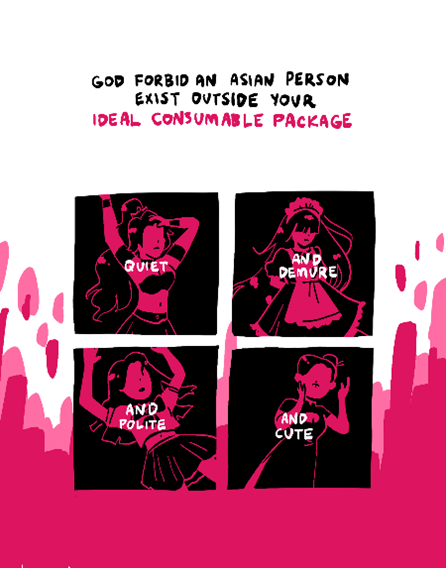
\includegraphics[width=8cm]{Picture1.png}
    \caption{Cultural Expectations of Asian Women}
    \label{fig:1}
\end{figure}
\begin{figure}
    \centering
    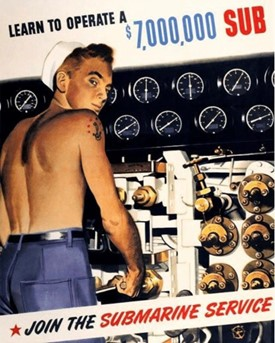
\includegraphics[width=8cm]{Picture2.jpg}
    \caption{Propaganda of a Sailor plays into homosexuality}
    \label{fig:enter-label}
\end{figure}

\section{Musical Artifact of a Queer Mariner}
This is what I will call my Annotated Discography, or my justification for why each of these songs belongs in this 'album', and what the intersection of the content of the music and of the people represented by my particular drag look means to me.
\subsection{Song: Off to Sea Once More\\
Costume: Sailor Moon}
	Off To Sea Once More is a song about the bitter cycle of a poor sailor’s life, and a depiction of the stereotype of his vices. Many young Jack Tars come home with their pockets full of money, only to blow it all on prostitutes and alcohol. Such proclivities are why in modern Hong Kong, still a central port as back in the golden age of wooden ships and iron men, Sailor’s Homes have a mission to keep those poor boys off the streets and from destroying themselves. Forgotten Spaces interviews the proprietor of that establishment, where he explains in no uncertain terms that setting up an internet café is the responsible alternative to allowing the sailors to go whoring as they wish. The song also presents a much less glamorous view of the seaman himself than almost any other song in my repertoire, or than by Jack Tar hero of Britain, or Popeye. He is Edward Barlow’s poor seaman. Also, casual misogyny for free in the outro verse: \say{It was then that I wished that I was dead or safe with the girls on shore. […] Take my advice: drink no strong drink, don’t go sleeping with no whore, get married instead and spend all night in bed and go to sea no more}\\
As explored in On the Waterfront, leaving the sea (and being a married man) are the death of the mariner. Both of those safe and peaceful lives with a Mrs. Jack Sprat mean that he stops being a seaman. 
	My costume choice as Sailor Moon is to be evocative of both halves of the second verse. “I spent the night with Angeline I was too drunk to roll in bed, me watch was new, me money too, in the morning with them she’d fled.” By audio I’m the sailor singing the song, but visually I’m Angeline who robbed him. Every old sailor you meet has some story about going whoring in some backwater Asian port and ‘accidentally’ tangling with, for instance, a Thai Ladyboy or a Filipino bakla. I represent both, but both are victims of the capitalist, “Rapper Brown” in the song. Who is also me because I own a few shares of stock in some hotel chains, where both Jack Sprat and Angeline can be found.
\subsection{Song Greenland Whale Fisheries\\
Costume: Blue work uniform}
	This song is very evocative of some passages from Moby Dick that are relevant to the theme of the project.
\begin{quote}
    \say{For God's sake, be economical with your lamps and candles! not a gallon you burn, but at least one drop of man's blood was spilled for it.} -The Affidavit
\say{As for the residue of the Pequod’s company, be it said, that at the present day not one in two of the many thousand men before the mast employed in the American whale fishery, are Americans born, though pretty nearly all the officers are. Herein it is the same with the American whale fishery as with the American army and military and merchant navies, and the engineering forces employed in the construction of the American Canals and Railroads. The same, I say, because in all these cases the native American literally provides the brains, the rest of the world as generously supplying the muscles.} -Knights and Squires
\end{quote}

This is a historical song about capitalism, which means that it is about race also. The climax of the song ends \begin{quote}
    The losing of seven fine seamen, it grieved our captain sore/ but the losing of our bloody sperm whale, it grieved him ten times more.
\end{quote}
The Filipino A/B in a blue boiler suit turns to for eight hours of day work and 4 hours of watch a day, he is the last to see any money, and the first to die in an explosion or sudden sinking of the vessel. The sperm whale is worth seventy times the life of the seaman, and although we no longer get our lamp oil from marine mammals, the explosion of a crude oil tanker costs the lives of a half a crew of seamen, but lowers the company’s share price by ten cents, therefore we’re a dime a dozen.
\subsection{Song: Transports and Old Baileys\\
Costume: Khakis}
The khaki uniform (perhaps reminiscent of Churchill’s Black and Tans?) is representative of power, authority, and the navy, the military, and the police. The history of Australia’s history as a British colony is that of a penal colony full of convicts as well as their jailers, who are just as far from home as the convicts. The distance from London to Sidney is 13000 miles via Cape of Good hope, and 90 days or more each way in a sailing ship. The seamen of the transports are thus condemned to a half year aboard a prison ship, but they work, but they are paid.
\subsection{Song: Bleacher Lassie of Kelvin Hall\\
Costume: Salt and Peppers}
This song is a ballad sang by one person, but the alternating verses have the singer change perspective between the sailor and his titular Lassie. The first time I ever sang this song, I was uncomfortable with this double identity of the singer, even though the original recording was sung by only a male voice. In rehearsal, I would hesitate audibly when in the second verse, ‘she’ replies with “oh indeed kind sir, and it’s the truth I’ll tell ye, I’m the bleacher lassie of Kelvin Hall” Of course, years later, I’m much more comfortable. This dual identity aspect also informs my costuming decision, my Salt and Pepper school uniform. The environment of the Maritime Academy is extremely masculine, and I’ve often felt that this school is so manly that even the women are men. It is a little act of rebellion that I wear the alternate uniform, even though it is now authorized for all genders (thank you Associated Students). The corps and the sea are all about conformity, and if I conform to an alternate standard, that’s still standing out. Even though the 50s style women’s navy uniform with skirt is emblematic as a more misogynistic time, even that bundles into the message of the song. I am now the sailor who will be gone years at a time, abandoning my lassie and having the moral expectation that she’ll continue to wait for me for years, and as soon as I come home, even if she can’t recognize me because my appearance is so changed by the sea and she scorns my advances thinking that I’m some other sailor, she’ll jump right back into my arms. I’m at sea a man and a woman ashore, and I’m sure that my family would choose not to recognize me if they saw me like this.
\subsection{Song: Topman and the Afterguard\\
Costume: Victorian Sailor}
In the song, the Topman asks the afterguard to pray with him and complain of the various misfortunes suffered on shipboard. The Boatswain beats the men, the Purser gives the sailors tiny portions of disgusting food, the officers don’t pay them, and there is not enough alcohol. In the modern day, many of these complaints have been addressed by the law. In 1850, the United States prohibited corporal punishment for sailors. Today’s seamen still complain that the food is not enough and not good enough, but revere the miracles that SUP stewards can manage. Even so, as I write this on the Training Ship, I can watch my friends wobble back and forth between “this mystery meat was almost like food today” and “I need more.” There is a fun historical connection between this song and the Spithead and Norr Mutinies, “the purser’s pound” was reckoned at 14 ounces. When provisioning the ship, the purser would buy a pound of beef, take two ounces off the top for his financial gain, and gives the remaining 14 ounces to the sailors or in practice, just purchases 87.5\% of the promised amount, and pockets the cash. Reforms to the royal navy after Spithead prohibited this practice. Ships are required to post a fo’c’s’le card detailing the pay scales for each position on the ship, and you can sue over unpaid wages. In the 21st century, alcohol is prohibited on all ships, as ships are both vehicles and heavy machinery, so it is forbidden to operate one while intoxicated. My costume is the Victorian Sailor rig that I wear for my part in the Dickens Fair Christmas Market. We sing old traditional songs as well as contemporary songs, the period to hit is any time that Dickens was alive. We must be true to the fiction of seamen that guests are aware of. This anachronism is to highlight the similarity and difference of the complaints of sailors present and past.
\subsection{Song: Nelson’s Death and Victory\\
Costume: Salt and Peppers}
The Salt and Pepper Costume is our way of pretending at the academy to have the military discipline that the commandants want us to believe is a good thing. This is as fictionalized as the era of wooden ships and iron men, a period much romanticized, and always frozen in time at the time of Nelson’s death and victory, the bifurcation points between the old ways and the new ways, the end of the threat of the French navy but before the United States civil war changed the nature of warfare all together. The act of this romanticization of the past is regressive, and those guys hate to see a boy in a skirt.
\subsection{Song: Leave Her Johnny\\
Costume: Blue work uniform}
This pump chantey is traditional both as the last song to be sung as the vessel is made fast in port as a final airing of grievances, and as a call to mutiny or desert the vessel. It is a list of complaints of poor treatment, foul weather, worse food, the sailor’s usual lot. Differently from the Topman and the Afterguard, I am in my work blues again. This all still is the case, but we now have hard hats. However, unlike in The Topman and the Afterguard, this song can also be sung in a sort of fond way. I have often remarked about the two kinds of fun, the kind that is enjoyable in the moment, and the kind that is enjoyable in hindsight. The effect of nostalgia can make you retroactively enjoy the backbreaking labor and hard driving bosun if you choose to remember more about weathering it with your friends. Or you can unionize.
\subsection{Song: Goodbye old Ship of Mine\\
Costume: Khakis}
I wear my school uniform khakis for this song because this song to me represents the end of singing in the maritime industry. Loving sea shanties kept kindled an interest in me of the sea, but when I came here to Cal Maritime, I found that all of that has been left behind because it’s not efficient clean and mechanical like ships are supposed to be. The heart of the sailor and the public image of a sailor is still in the days of wooden ships and iron men. We’re businessmen in suits now, and her name will only live on until the day I’m gone...
\subsection{Song: Mary Ellen Carter\\
Costume: Sailor Moon}
Mary Ellen Carter is one of Stan Roger’s most celebrated original songs, from the perspective of a crew member collaborating with friends to raise their old sunken ship. This song, although contemporary, is emblematic of a sailor’s feelings towards their vessel, a refuge in the inhospitable sea. \say{We couldn’t leave her there, you see, to crumble into scale. She saved our lives so many times, living through the gale.} This song is also performed in memory of Stan at numerous shanty sing events internationally, including the one I regularly participate in with the San Francisco Maritime National Park.
The final stanzas are a hopeful message to those who have experienced massive trauma and hardship, to encourage them to persevere when all is lost. In an interview given by Bob Cusick, one of the three survivors of the Marine Electric Disaster, recalls pushing through the hypothermia by singing the last verse of this song while being pounded by waves, clinging desperately to a lifeboat for many hours until the Coast Guard arrived. In our Cargo Vessel Operations class, although we covered the SS Marine Electric, this part of the story was omitted, much the way that maritime song is omitted from our school.
As for the personal message, I’d like to dedicate this song to the struggle of queer people. The AIDS crisis, the recent wave of transphobic laws being enacted, being kicked out of their parents’ homes, being fired from jobs, discrimination, and other suffering I can’t even imagine. “You, to whom adversity has dealt the final blow, with smiling bastards lying to you everywhere you go, turn to and put out all your strength of arm and heart and brain and like the Mary Ellen Carter, rise again! Though your heart it be broken, and life about to end; no matter what you’ve lost, be it a home, a love a friend, like the Mary Ellen Carter rise again!” For the first time on this album, my decision to wear drag is not as a dichotomy, but as a synthesis, that I can represent maritime for the queer community, queers for the maritime community, and the joy of sea music for both. Sailor Moon is the center of that Venn Diagram.

\subsection{Narrative of Track Order} Our  story begins at its ending. Our sailor has returned from sea with his pockets full, but emptied again must go again. He is put to work in the Greenland whale fisheries where he witnesses seven friends die. He is impressed into the navy. On a voyage to transport prisoners to the far side of the globe, he is as much a prisoner of the ship as any of the convicts. He recalls a girl he left behind in Scotland, who promised to wait for him to come back to marry him, even if it takes 14 years. He continues at sea, complaining about the rotten treatment and delayed pay. The battle of Trafalgar takes place. He is permitted to leave and sings the meanest song he can about his ship before quitting her. The ship is sold out of the service, lives for a few years as a merchantman, but at the end of her useful life, he sees her being broken up for firewood. He is overcome with sentiment he didn’t know he felt. Even to entertain a fantasy of refloating the Mary Ellen Carter. But he doesn’t have that kind of money, in fact, his money is all gone, and he must Go to Sea Once More.


\end{document}
